\clearpage
\begin{appendices}

\chapter{Principal Component Analysis} \label{app:pca}
Descriptors should be as discriminative as possible, whilst also being as compact as possible. This means that each descriptor should encode encode as much information allowing it to be differentiated from other images as possible, whilst also containing the minimum amount of data allowing it to do this. The descriptors investigated in the main body of the report focus on creating discriminative descriptors, but do not place as much importance on generating compact descriptors. It is possible that many of the descriptors contain information which is common to all images, and therefore acts as wasted data.

\Gls{pca} analyses these descriptors and, via construction of an eigenmodel, allows for them to be projected into a lower dimensional space. This discards the `wasted' data in the descriptors.

Figures \ref{fig:pca-grid-color-sheep} and \ref{fig:pca-grid-color-books} show the results of projecting the descriptors into a lower dimensional space.  The $E$ value refers to the proportion of total eigenvalue energy to preserve. Eigenvalue energy is equal to the sum of all of the Eigenvalues which make up the descriptor. Therefore, for $E=0.5$, the sum of the eigenvalues of the dimensions which the data is projected into, is greater than or equal to half of the total sum of the eigenvalues.


\begin{figure}[ht]
	\begin{minipage}[]{0.3\linewidth}
		\centering
		\includegraphics[width = 0.9\linewidth]{figs/msrc/9_23_s}
		\subcaption{Query image}
	\end{minipage}
	\begin{minipage}[]{0.7\linewidth}
		\centering
		\begin{tikzpicture}
		\prplot{data/pca/grid_color_hist/9_23_s/pr_1.txt}{E=0.1}
		\prplotadd{data/pca/grid_color_hist/9_23_s/pr_3.txt}{E=0.3}
		\prplotadd{data/pca/grid_color_hist/9_23_s/pr_5.txt}{E=0.5}
		\prplotadd{data/pca/grid_color_hist/9_23_s/pr_7.txt}{E=0.7}
		\prplotadd{data/pca/grid_color_hist/9_23_s/pr_9.txt}{E=0.9}
		\prplotadd{data/pca/grid_color_hist/9_23_s/pr_9.9.txt}{E=0.99}
		\prplotadd{data/pca/grid_color_hist/9_23_s/pr_11.txt}{No PCA}
		\prplotadd{data/gridding/color_hist/9_23_s/pr_2.txt}{No EM}
		\prplotclose
		\end{tikzpicture}
		\subcaption{Resultant graph}
	\end{minipage}
	\caption{Gridded RGB histogram, using PCA for query image 9\_23\_s}
	\label{fig:pca-grid-color-sheep}
\end{figure}

\begin{figure}[ht]
	\begin{minipage}[]{0.3\linewidth}
		\centering
		\includegraphics[width = 0.9\linewidth]{figs/msrc/13_1_s}
		\subcaption{Query image}
	\end{minipage}
	\begin{minipage}[]{0.7\linewidth}
		\centering
		\begin{tikzpicture}
		\prplot{data/pca/grid_color_hist/13_1_s/pr_1.txt}{E=0.1}
		\prplotadd{data/pca/grid_color_hist/13_1_s/pr_3.txt}{E=0.3}
		\prplotadd{data/pca/grid_color_hist/13_1_s/pr_5.txt}{E=0.5}
		\prplotadd{data/pca/grid_color_hist/13_1_s/pr_7.txt}{E=0.7}
		\prplotadd{data/pca/grid_color_hist/13_1_s/pr_9.txt}{E=0.9}
		\prplotadd{data/pca/grid_color_hist/13_1_s/pr_9.9.txt}{E=0.99}
		\prplotadd{data/pca/grid_color_hist/13_1_s/pr_11.txt}{No PCA}
		\prplotadd{data/gridding/color_hist/13_1_s/pr_2.txt}{No EM}
		\prplotclose
		\end{tikzpicture}
		\subcaption{Resultant graph}
	\end{minipage}
	\caption{Gridded RGB histogram, using PCA for query image13\_1\_s}
	\label{fig:pca-grid-color-books}
\end{figure}

Both Figures \ref{fig:pca-grid-color-sheep} and \ref{fig:pca-grid-color-books} show the expected result that, the higher the value of $E$, the better the performance of the distance measure. The `No \glsentryshort{pca}' plot shows the result of generating the eigenmodel and projecting the descriptors into this space, but without reducing the dimensionality of the descriptor. This plot is identical to the `No EM' plot, which is the results obtained without projecting the descriptors into the eigenmodel space. This is the expected result since, if all dimensions are maintained, the data has not been changed, and the Euclidean distance between descriptors in the two spaces should be identical.

Table \ref{tbl:pca-dim-red} shows the number of dimensions in the resultant descriptors when performing \gls{pca} on a gridded global colour histogram at different energy values. The table shows that even for $E=0.99$, i.e. 99 \% of the total eigenvalue engery, the descriptor dimensions can be reduced from 384 dimensions to 104. This shows that there are many dimensions with almost no variation in the original descriptor space which can be removed without reducing performance by a large amount. This is demonstrated in the test data, where the plot for $E=0.99$ is almost identical to the plot for `No \glsentryshort{pca}'. This reduces the size of the descriptor to only 26\% of it's size without \gls{pca}. Reducing the value of $E$ even further to $0.9$ means that the descriptor is only 8.9\% of its original size, whilst still maintaining good performance.

\begin{table}[ht]
	\rowcolors{2}{gray!25}{white}
	\caption{\glsentryshort{pca} Dimension reduction for Gridded RGB Histogram}
	\label{tbl:pca-dim-red}
	\centering
	\pgfplotstabletypeset[
	col sep=comma,
	string type,
	columns/e/.style={column name={\textbf{Energy}}, column type={r}},
	columns/dims/.style={column name={\textbf{\shortstack{Descriptor\\dimensions}}}, column type={r}},
	columns/percent/.style={column name={\textbf{\shortstack{Proportion of\\total dimensions}}}, column type={r}},
	every head row/.style={before row=\toprule, after row=\midrule},
	every last row/.style={after row=\bottomrule},
	]{data/pca/grid_color_hist/dim_report.txt}
\end{table}

\chapter{Distance Measures} \label{app:dist-measures}

The results presented in the body of this report use the L2 Norm, otherwise known as Euclidean distance, to measure the distance between descriptors. However despite this being the most common choice for distance measure, other distance measures do exist, these will be compared in this Appendix.

The distance measured investigated are:
\begin{enumerate}
	\item $L_1$ norm (Manhattan distance)
	\item $L_2$ norm (Euclidean distance)
	\item $L_2$ norm squared
	\item $L_\infty $ norm (Chebyshev distance)
	\item Mahalanobis distance
\end{enumerate}

A vector norm, $|\mathbf{x}|$ refers to a scaler property that, in perhaps an abstract way, describes the length of a vector, $\mathbf{x}$. Mathematically this is defined as shown in Equation \ref{eq:norm-def} \cite[p. 1081]{gradshteyn2007}.
\begin{align}
|\mathbf{x}| > 0 \quad &\text{when } \mathbf{x} \neq \mathbf{0} \nonumber \\
|\mathbf{x}| = 0 \quad &\text{when } \mathbf{x} = \mathbf{0} \nonumber \\
|k\mathbf{x}| = |k||\mathbf{x}| \quad &\text{for any scalar } k \nonumber \\
|\mathbf{x}+\mathbf{y}| \geq |\mathbf{x}|+|\mathbf{y}| \quad & \label{eq:norm-def}
\end{align}

The $L_1$, $L_2$ and $L_3$ norms describe this distance in different ways. The $L_2$ norm is the most common norm because it describes the point to point distance in Euclidean geometry. It is defined in Equation \ref{eq:L2-norm-def} \cite[p.1081]{gradshteyn2007}.

\begin{equation}
|\mathbf{x}|_2 = \sqrt{\sum_{r=1}^{n} |x_r|^2} \quad \text{where } \mathbf{x} = [ x_1 , x_2, ... , x_n] \label{eq:L2-norm-def}
\end{equation}

The $L_1$ norm describes distance in a slightly different way. It is the sum of the magnitudes of the vector components. This is the reason it is given the name `Manhattan' or `city block' distance, because in a two dimensional vector space, the $L_2$ norm would be the hypotenuse of a right angle triangle joining two nodes, whilst the $L_1$ norm would be the sum of the other two sides, analogous to walking along city blocks to go between two points. It is defined in Equation \ref{eq:L1-norm-def} \cite[p.1081]{gradshteyn2007}.

\begin{equation}
|\mathbf{x}|_1 = \sum_{r=1}^{n} |x_r| \quad \text{where } \mathbf{x} = [ x_1 , x_2, ... , x_n] \label{eq:L1-norm-def}
\end{equation}

The $L_\infty $ norm describes distance as the magnitude of the largest component of the vector. This therefore ignores the magnitudes of all smaller components. It is defined in Equation \ref{eq:L-inf-norm-def} \cite[p.1081]{gradshteyn2007}.

\begin{equation}
|\mathbf{x}|_\infty = \max_{i} |x_i| \quad \text{where } \mathbf{x} = [ x_1 , x_2, ... , x_n] \label{eq:L-inf-norm-def}
\end{equation}

These norms can be summarised in one equation which can define the $L_p$ norm for any $p$. However using the $L_p$ norm for values other than $p=1,2,\infty$ is not common.
\begin{equation}
|\mathbf{x}|_p = \sqrt[p]{\sum_{r=1}^{n} |x_r|^p} \quad \text{where } \mathbf{x} = [ x_1 , x_2, ... , x_n] \label{eq:Lp-norm-def}
\end{equation}

The only other distance measures under consideration are the $L_2$ norm squared, and the Mahalanobis distance. The $L_2$ norm squared is equal to the $L_2$ norm definition, but only the sum of the squared components is considered, this sum is not square rooted. This measure therefore places an increasing weight on larger components, as they will contribute a larger amount to the sum compared to their contribution to the square root of the number.

The Mahalanobis distance is slightly different to the other distance measures presented. Instead of considering distance as a function of the differences between different vector dimensions in a standard Euclidean space, the Mahalanobis distance instead first calculates the spread of the data in each dimension, and then measures difference in terms of how many standard deviations each linear difference represents. This can provide a normalising factor to the difference function because a difference in a dimension with a large spread of data will represent a much smaller contribution than the same linear difference in a dimension with a small spread. This effect can be thought of as the distance function fitting itself to the shape of the data. The Mahalanobis distance is implemented in the system by weighting the Euclidean distance with the eigenvalue for that dimension. This is shown mathematically in Equation \ref{eq:mahan-def}, where $v_r$ represents the eigenvalue for each dimension.

\begin{equation}
|\mathbf{x}|_2 = \sqrt{\sum_{r=1}^{n} \frac{|x_r|^2}{v_r} } \quad \text{where } \mathbf{x} = [ x_1 , x_2, ... , x_n] \label{eq:mahan-def}
\end{equation}

\begin{figure}[ht]
	\begin{minipage}[]{0.3\linewidth}
		\centering
		\includegraphics[width = 0.9\linewidth]{figs/msrc/9_23_s}
		\subcaption{Query image}
	\end{minipage}
	\begin{minipage}[]{0.7\linewidth}
		\centering
		\begin{tikzpicture}
		\prplot{data/dist_measure/9_23_s/pr_L1.txt}{$L_1$ norm}
		\prplotadd{data/dist_measure/9_23_s/pr_L2.txt}{$L_2$ norm}
		\prplotadd{data/dist_measure/9_23_s/pr_L2_sq.txt}{$L_2$ norm squared}
		\prplotadd{data/dist_measure/9_23_s/pr_L_Inf.txt}{$L_\infty $ norm}
		\prplotadd{data/dist_measure/9_23_s/pr_Mahal.txt}{Mahalanobis distance}
		\prplotclose
		\end{tikzpicture}
		\subcaption{Resultant graph}
	\end{minipage}
	\caption{Gridded RGB histogram results for query image 9\_23\_s}
	\label{fig:dist-meas-sheep}
\end{figure}

\begin{figure}[ht]
	\begin{minipage}[]{0.3\linewidth}
		\centering
		\includegraphics[width = 0.9\linewidth]{figs/msrc/13_1_s}
		\subcaption{Query image}
	\end{minipage}
	\begin{minipage}[]{0.7\linewidth}
		\centering
		\begin{tikzpicture}
		\prplot{data/dist_measure/13_1_s/pr_L1.txt}{$L_1$ norm}
		\prplotadd{data/dist_measure/13_1_s/pr_L2.txt}{$L_2$ norm}
		\prplotadd{data/dist_measure/13_1_s/pr_L2_sq.txt}{$L_2$ norm squared}
		\prplotadd{data/dist_measure/13_1_s/pr_L_Inf.txt}{$L_\infty $ norm}
		\prplotadd{data/dist_measure/13_1_s/pr_Mahal.txt}{Mahalanobis distance}
		\prplotclose
		\end{tikzpicture}
		\subcaption{Resultant graph}
	\end{minipage}
	\caption{Gridded RGB histogram results for query image 13\_1\_s}
	\label{fig:dist-meas-books}
\end{figure}

Figures \ref{fig:dist-meas-sheep} and \ref{fig:dist-meas-books} show the results of applying different distance measures to two test images. In both cases the $L_2$ norm squared has performed exactly as well as the $L_2$ norm. This is an interesting result, it implies that, in the test data, no matrix dimension difference magnitude had a much larger magnitude than the other significant dimensions.

The results for the $L_1$ norm and $L_\infty$ norm showed much greater difference in the test using image 13\_1\_s than 9\_23\_s. It can be seen that whilst the $L_1$ and $L_2$ norm showed generally similar performance, the $L_\infty$ norm showed significantly poorer performance. This confirms that only considering the most significant vector dimension is not sufficient to accurately determine differences between the images. The $L_2$ norm also outperformed the $L_1$ norm in the average case for the books. The image of the sheep however showed similar performance between distance measures.

The Mahalanobis distance performed very poorly for image 13\_1\_s, which is a surprising result. This implies that it representing difference in terms of the standard deviations moved, rather than linear distance, does not translate well into the output of the descriptor.

It is worth noting that Figures \ref{fig:dist-meas-sheep} and \ref{fig:dist-meas-books} were performed on descriptors which had had an eigenmodel generated from them, and then had the descriptors projected into that space. This was performed in order to allow the Mahalanobis distance to be compared also. However one effect this had is that it artificially increased the performance of the $L_\infty$ norm. The $L_\infty$ norm only compares the largest dimension of difference between two points, therefore when the descriptors are projected into the eigenmodel space, the direction of largest variation is aligned with the first dimension of the descriptor. This gives the $L_\infty$ norm will often use this dimension of largest variation as its differentiator, leading to artificially higher results than if the descriptors were naturally aligned with the dimensions. This is illustrated in Figure{fig:dist-meas-nopca-books}.


\begin{figure}[ht]
	\begin{minipage}[]{0.3\linewidth}
		\centering
		\includegraphics[width = 0.9\linewidth]{figs/msrc/13_1_s}
		\subcaption{Query image}
	\end{minipage}
	\begin{minipage}[]{0.7\linewidth}
		\centering
		\begin{tikzpicture}
		\prplot{data/dist_measure/13_1_s/pr_L_Inf.txt}{$L_\infty $ norm}
		\prplotadd{data/dist_measure_no_pca/13_1_s/pr_L_Inf.txt}{$L_\infty $ norm (No EM)}
		\prplotclose
		\end{tikzpicture}
		\subcaption{Resultant graph}
	\end{minipage}
	\caption{Gridded RGB histogram results for query image 13\_1\_s}
	\label{fig:dist-meas-nopca-books}
\end{figure}


\chapter{Test Methodology} \label{app:test-methodology}
In order to test the system, a unit test has been written for all of the descriptor and distance measure functions, as well as several other key functions. Each of these tests complies with \gls{matlab}'s unit testing framework, so can be executed using the \texttt{runtests} command. A description of the tests for each function is detailed in Table \ref{tbl:list-of-tests}.

\begin{table}[h]
	\rowcolors{2}{gray!25}{white}
	\centering
	\caption{List of tests implemented}
	\label{tbl:list-of-tests}
	\begin{tabular}{ l p{0.6\linewidth} }
		\toprule
		\bfseries Function Tested & \bfseries Tests implemented \\
		\midrule
		\texttt{vs\_compute\_histogram} &
		\begin{minipage}[t]{\linewidth}
			\begin{itemize}[leftmargin=*]
				\item Two tests against manually calculated data sets.
			\end{itemize}
		\end{minipage} \\
%		
		\texttt{vs\_compute\_rgb\_histogram} &
		\begin{minipage}[t]{\linewidth}
			\begin{itemize}[leftmargin=*]
				\item Four tests against test images with known colour distributions, against manually calcualated histograms.
			\end{itemize}
		\end{minipage} \\
%		
		\texttt{vs\_construct\_eigenmodel} &
		\begin{minipage}[t]{\linewidth}
			\begin{itemize}[leftmargin=*]
				\item Test eigenmodel dimensions and against Eigen\_Build.
				\item Test projected descriptors against Eigen\_Project.
				\item Test \gls{pca} applied eigenmodel against Eigen\_Deflate.
				\item Test \gls{pca} applied projected descriptors against Eigen\_Project.
			\end{itemize}
		\end{minipage} \\
%		
		\texttt{vs\_edge\_detect} &
		\begin{minipage}[t]{\linewidth}
			\begin{itemize}[leftmargin=*]
				\item Test operation against library function with three test images.
				\item Test operation against library function for a sample image.
			\end{itemize}
		\end{minipage} \\
%		
		\texttt{vs\_grid} &
		\begin{minipage}[t]{\linewidth}
			\begin{itemize}[leftmargin=*]
				\item Test 1x1 grid output using computation function that returns entire image.
				\item Test 2x2 grid output using computation function that returns entire image.
			\end{itemize}
		\end{minipage} \\
%		
		\texttt{vs\_L1\_norm} &
		\begin{minipage}[t]{\linewidth}
			\begin{itemize}[leftmargin=*]
				\item Test output of zero vector against itself.
				\item Test output of random vector against itself. 
				\item Test two manually calculated results.
				\item Test against library function for random vectors.
			\end{itemize}
		\end{minipage} \\
%		
		\texttt{vs\_L\_Inf\_norm} &
		\begin{minipage}[t]{\linewidth}
			\begin{itemize}[leftmargin=*]
				\item Test output of zero vector against itself.
				\item Test output of random vector against itself. 
				\item Test two manually calculated results.
				\item Test against library function for random vectors.
			\end{itemize}
		\end{minipage} \\
%		
		\texttt{vs\_L\_2\_norm} &
		\begin{minipage}[t]{\linewidth}
			\begin{itemize}[leftmargin=*]
				\item Test output of zero vector against itself.
				\item Test output of random vector against itself. 
				\item Test two manually calculated results.
				\item Test against library function for random vectors.
			\end{itemize}
		\end{minipage} \\
%		
		\texttt{vs\_L\_2\_norm\_squared} &
		\begin{minipage}[t]{\linewidth}
			\begin{itemize}[leftmargin=*]
				\item Test output of zero vector against itself.
				\item Test output of random vector against itself. 
				\item Test two manually calculated results.
				\item Test against library function for random vectors.
			\end{itemize}
		\end{minipage} \\
%		
		\texttt{vs\_mahalanobis\_distance} &
		\begin{minipage}[t]{\linewidth}
			\begin{itemize}[leftmargin=*]
				\item Test output of zero vector against itself.
				\item Test output of random vector against itself. 
				\item Test three manually calculated results.
			\end{itemize}
		\end{minipage} \\
		\bottomrule
	\end{tabular}
\end{table}


	

\section{Test pattern generation} \label{sec:test-pattern-gen}
Some tests require test patterns in order to test their functionality correctly. For this purpose a suite of test pattern generation programs was written to create image which contain:
\begin{itemize}
	\item A uniform colour.
	\item A uniform pattern.
	\item A combination of the above.
	\item A grid of several of the above images.
\end{itemize}
These test patterns are used internally to the unit tests, as well as to perform system level testing.

A sample of the test images is shown in Figure \ref{fig:example-test-images}

\begin{figure}[ht]
	\begin{minipage}[]{0.5\linewidth}
		\centering
		
\includegraphics[width = 0.6\linewidth]{figs/test_imgs/color_5}
		\subcaption{A uniform colour test image}
	\end{minipage}
	\begin{minipage}[]{0.5\linewidth}
		\centering
		
\includegraphics[width = 0.6\linewidth]{figs/test_imgs/freq_1}
		\subcaption{A uniform pattern test image}
	\end{minipage}
	
	\begin{minipage}[]{0.5\linewidth}
		\centering
		
\includegraphics[width = 0.6\linewidth]{figs/test_imgs/color_cat_1}
		\subcaption{A grid of uniform colour images}
	\end{minipage}
	\begin{minipage}[]{0.5\linewidth}
		\centering
		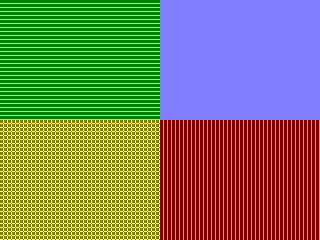
\includegraphics[width = 0.6\linewidth]{figs/test_imgs/color_freq_cat_4}
		\subcaption{A grid of transposed colour and pattern test images}
	\end{minipage}
	\caption{Example test images}
	\label{fig:example-test-images}
\end{figure}


\end{appendices}